\let\negmedspace\undefined
\let\negthickspace\undefined
\documentclass[journal]{IEEEtran}
\usepackage[a5paper, margin=10mm, onecolumn]{geometry}
%\usepackage{lmodern} % Ensure lmodern is loaded for pdflatex
\usepackage{tfrupee} % Include tfrupee package

\setlength{\headheight}{1cm} % Set the height of the header box
\setlength{\headsep}{0mm}     % Set the distance between the header box and the top of the text

\usepackage{gvv-book}
\usepackage{gvv}
\usepackage{cite}
\usepackage{amsmath,amssymb,amsfonts,amsthm}
\usepackage{algorithmic}
\usepackage{graphicx}
\usepackage{textcomp}
\usepackage{xcolor}
\usepackage{txfonts}
\usepackage{listings}
\usepackage{enumitem}
\usepackage{mathtools}
\usepackage{gensymb}
\usepackage{comment}
\usepackage[breaklinks=true]{hyperref}
\usepackage{tkz-euclide} 
\usepackage{listings}
% \usepackage{gvv}                                        
\def\inputGnumericTable{}                                 
\usepackage[latin1]{inputenc}                                
\usepackage{color}                                            
\usepackage{array}                                            
\usepackage{longtable}                                       
\usepackage{calc}                                             
\usepackage{multirow}                                         
\usepackage{hhline}                                           
\usepackage{ifthen}                                           
\usepackage{lscape}


\renewcommand{\thefigure}{\theenumi}
\renewcommand{\thetable}{\theenumi}
\setlength{\intextsep}{10pt} % Space between text and floats

\numberwithin{equation}{enumi}
\numberwithin{figure}{enumi}
\renewcommand{\thetable}{\theenumi}	

% Marks the beginning of the document
\begin{document}
\bibliographystyle{IEEEtran}

\title{9-9.3-6}
\author{EE24BTECH11049 \\ Patnam Shariq Faraz Muhammed}

% \maketitle
% \newpage
% \bigskip
{\let\newpage\relax\maketitle}

\textbf{QUESTION} \\
    Using integration, find the area of the region enclosed by the curve $y = x^2$ , the $x-axis$ and the ordinates $x = - 2$ and $x = 1$.\\
\textbf{SOLUTION:} \\
    \begin{table}[h!]    
      \centering
      \begin{tabular}[4pt]{| c| c|}
\hline 
    \textbf{FUNCTION} & \textbf{FORMULA} \\
\hline
    $g\brak{x}$ & $\vec{x^TVx}+\vec{2u^Tx}+f=0$\\
\hline
    The points of intersection & $ L: \vec{x} = \vec{h} + \kappa\vec{m},  \kappa \in \mathbb{R} $\\ of the line L with the conic &  $ \kappa_i = \frac{1}{\vec{m^TVm}}\brak{\vec{-m^T\brak{Vh+u}} \pm \sqrt{\sbrak{\vec{m^T\brak{Vh+u}}^2} - g(\vec{h})\brak{\vec{m^TVm}}}} $ \\section as above are \\given by $ \vec{x}_i = \vec{h} + \kappa_i\vec{m} $  \\  \\  
\hline
\end{tabular}


      \label{table: 9-9.3-6}
    \end{table}\\

    \begin{table}[h!]    
      \centering
      \begin{tabular}[4pt]{|c|}
    \hline 
    \textbf{DESCRIPTION}\\
    \hline
    $\vec{V} = \norm{n}^2\vec{I} - e^2\vec{nn^T}$ \\
    $\vec{u} = ce^2\vec{n} - \norm{n}^2\vec{F}$ \\
    $f = \norm{n}^2\norm{F}^2 - c^2e^2 $ \\
    \hline
    
\end{tabular}

      \caption{Variables Used}
      \label{table: 9-9.3-6}
    \end{table}
    Substituting the given values, we have \\
\begin{align}
	\vec{V} &= \myvec{ 0 & 0 \\ 0 & 1 } \\
	\vec{u} &= \myvec{ \frac{-1}{2} \\ 0 } \\
	f &= 0 
\end{align}\\
Substituting the values, we get the point of intersection as \\
\begin{align}
	\kappa_i &= -\myvec{0 \\ 1}\myvec{\frac{-1}{2} & 0} \pm \sqrt{\sbrak{\myvec{0 & 1}\myvec{ \frac{-1}{2} \\ 0} }^2 + 1\brak{1}} \\
	\kappa_i &= 1 
\end{align}\\
Hence, the point of intersection is \myvec{ 1 \\ 1} \\
Similarly, the other point is given by \myvec{ -2 \\ 4 } .\\
The area bounded by the curve and the line is \\
\begin{align}
	\int_{-2}^{1} \brak{x^2} dx &= \frac{1}{3}\brak{ 1 - (-8) } \\
	&= 3 
\end{align}\\
Hence the required area is $3$ .
	
\begin{figure}[ht]
	\centering
	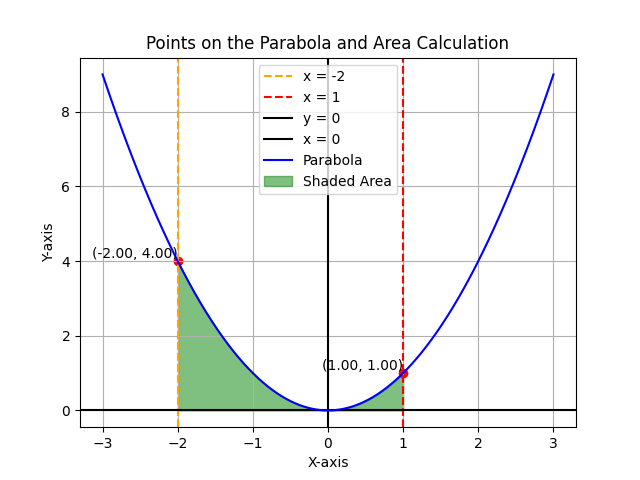
\includegraphics[width=0.8\textwidth]{figs/fig.png}
	\caption{A plot of the given question.}
\end{figure}
\end{document}
